\documentclass{article}
\usepackage[section]{placeins}
\usepackage{graphicx, wrapfig, amsmath, amssymb, physics, hyperref}
\hypersetup{
    colorlinks=true,
    linkcolor=blue,
    filecolor=magenta,      
    urlcolor=cyan,
    }

\author{Yaghoub Shahmari}
\title{Report - Problem Set No 6}
\date{\today}
\graphicspath{ {../Figs/} }

\begin{document}
    \maketitle
    \section*{Problem 1}
    \textbf{Basic description:}

    In this problem, we're going to find the answer to the integral of a function.
    So we will follow the instructions introduced by the book.
    We will deploy both methods of the Monte Carlo algorithm for solving an integration.
    As the problem told us:

    $$f_{(x)} = \int e^{-x^2} \mathop{dx} \Rightarrow I = \int_0^2 e^{-x^2} \mathop{dx} = \frac{\sqrt{\pi}}{2} \mathrm{erf}_{(2)}$$
    
    We solved the integration for different amounts of samples for both methods
    and showed the benchmark result of each one in the notebook (Q1-1DInt.ipynb).
    We also showed the distribution of answers for both methods.
    And finally, we will show the answers, errors, and performance for each amount of samples.

    \textbf{The results:}

    \begin{figure}[!htb]
        \centering
        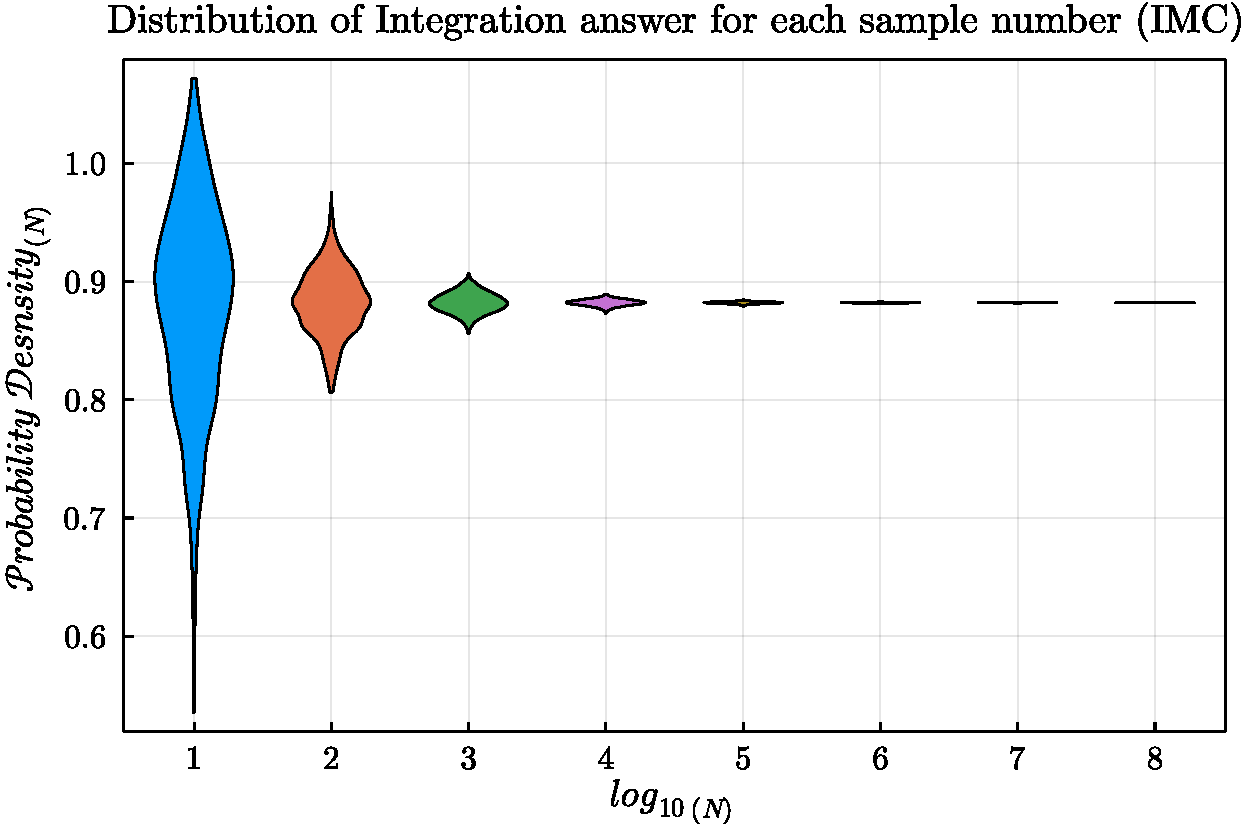
\includegraphics[scale = 0.25]{/Q1/IMCVilPlot}
        \label{fig:1.1}
        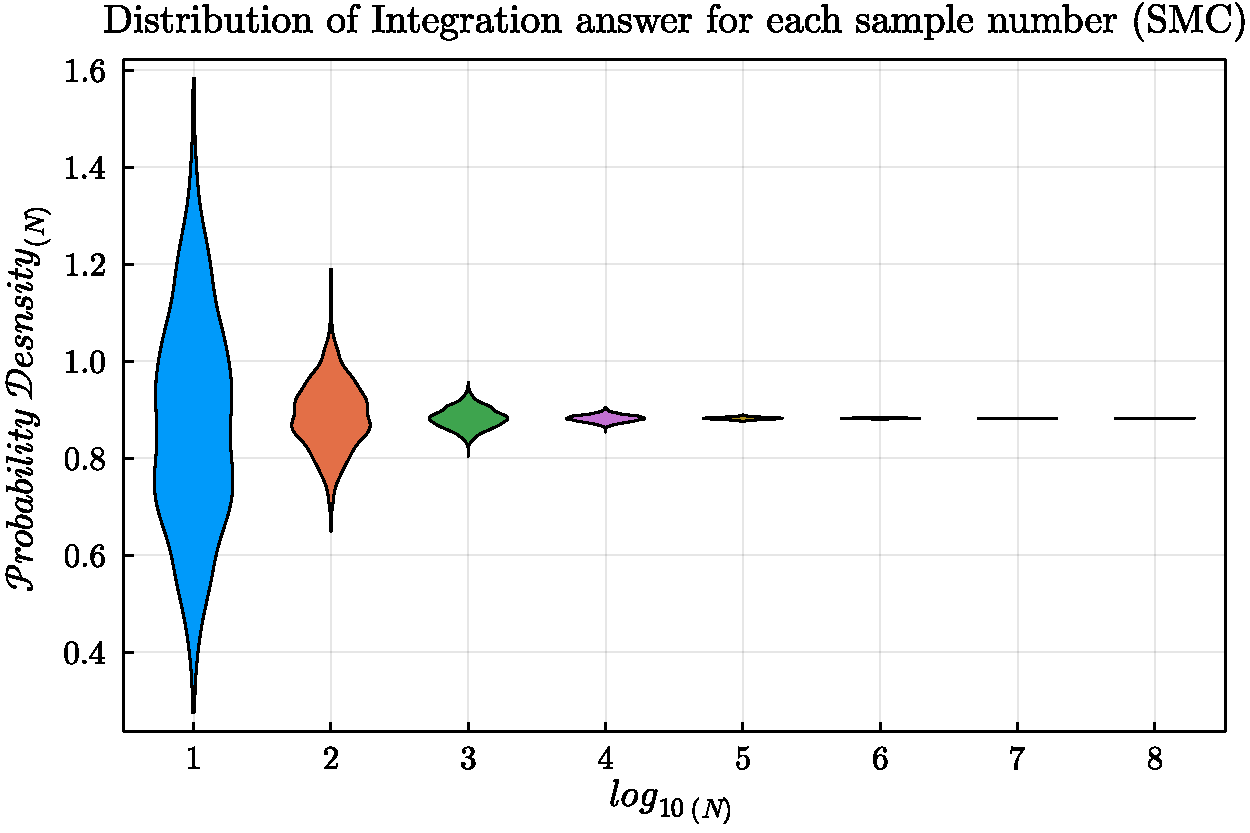
\includegraphics[scale = 0.25]{/Q1/SMCVilPlot}
        \label{fig:1.2}
        \caption{Distribution of answers for both methods.}
    \end{figure}

    \begin{figure}[!htb]
        \centering
        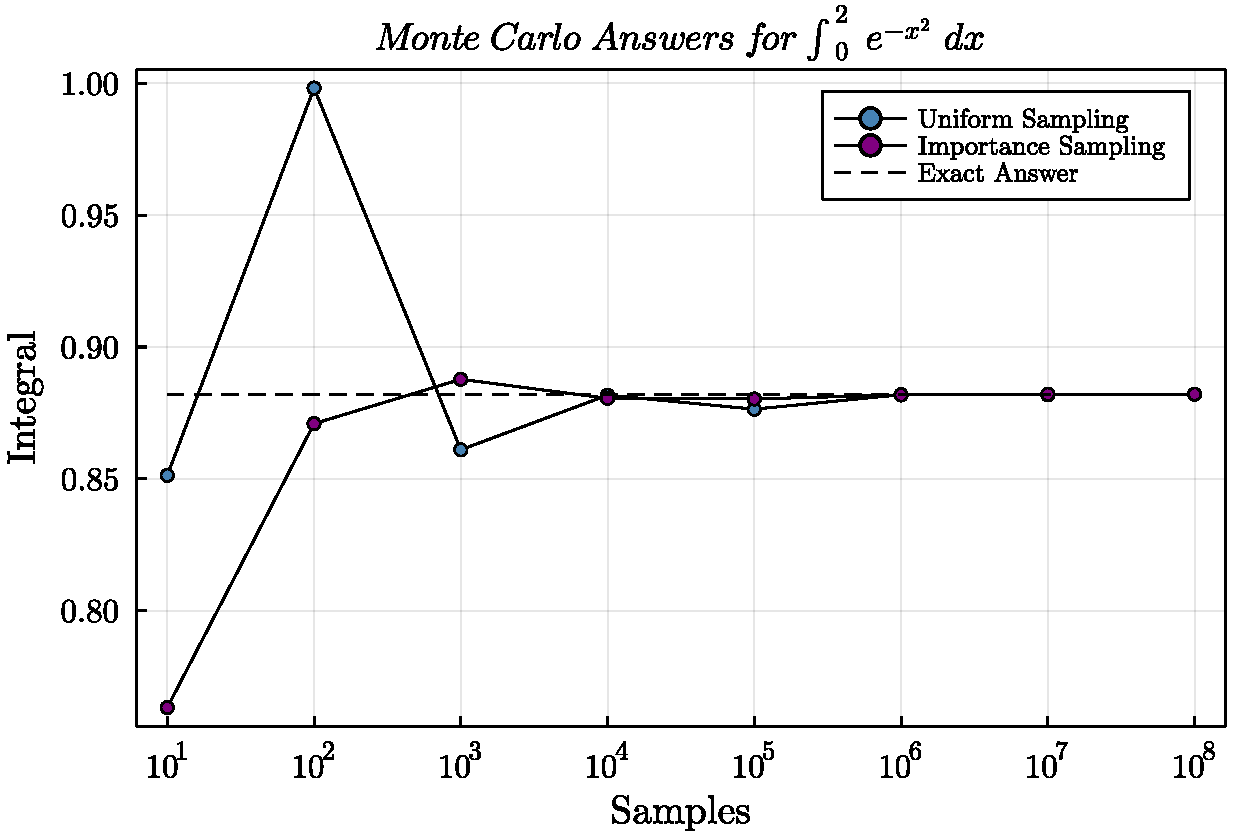
\includegraphics[scale = 0.42]{/Q1/MCAnswerPlot}
        \label{fig:1.3}
        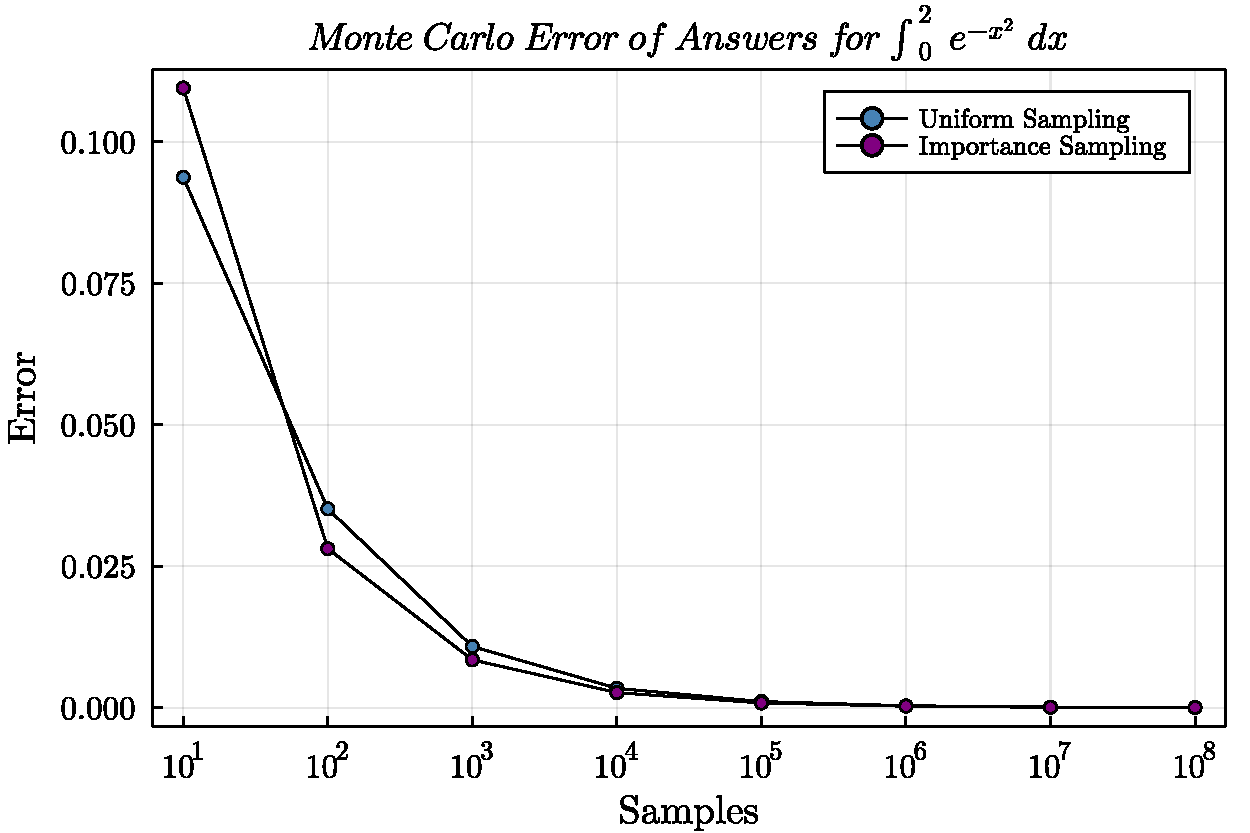
\includegraphics[scale = 0.42]{/Q1/MCErrorPlot}
        \label{fig:1.4}
        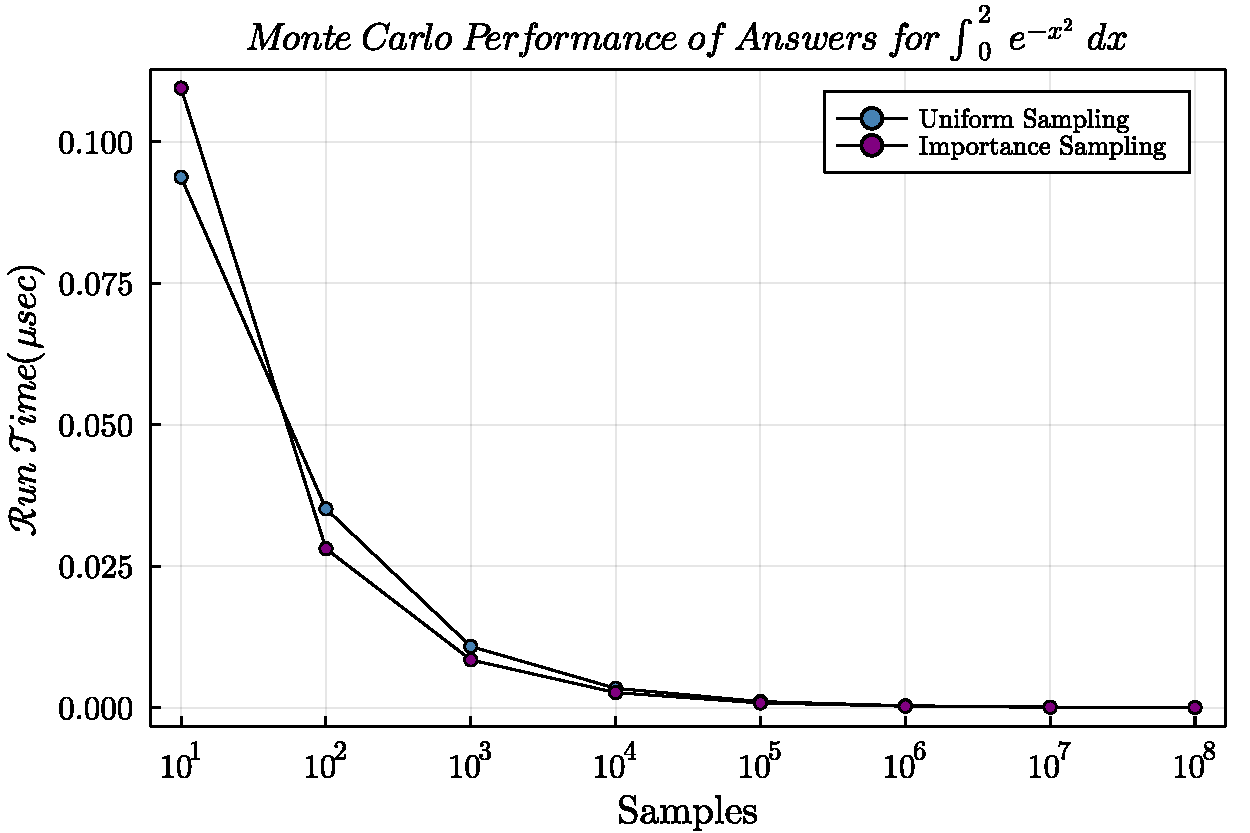
\includegraphics[scale = 0.42]{/Q1/MCPerformPlot}
        \label{fig:1.5}
        \caption{Plot of answers, errors, and performance for both methods.}
    \end{figure}

    \pagebreak

    \section*{Problem 2}
    \textbf{Basic description:}

    In this problem, we want to find the center of mass of
    a sphere whit specific mass distribution.
    So we have to find the answer to a 2D integration.
    As we know:

    $$R_{CoM} = \frac{I}{M} \Rightarrow R_{CoM} = \frac{\int_{Sphere} z \rho dV}{\int_{Sphere} \rho dV},\ \rho = \rho_0 (3 + \frac{r}{R} \cos{\theta}) \Rightarrow$$
    $$ R_{CoM} = \frac{\int_0^R\int_0^\pi (3+\frac{r}{R}\cos{\theta})r^3\sin{\theta}\cos{\theta} d\theta dr}{\int_0^R\int_0^\pi (3+\frac{r}{R}\cos{\theta})r^2\sin{\theta} d\theta dr}$$

    That has the exact answer of $R_{CoM} = \frac{R}{15}$.
    We drew the distribution of a bunch of answers.
    Also, we calculated the values of errors.
    The final answer is $R_{CoM} = 0.0665806190158467$.
    All steps and values are available in the notebook.

    \textbf{The results:}

    \begin{figure}[!htb]
        \centering
        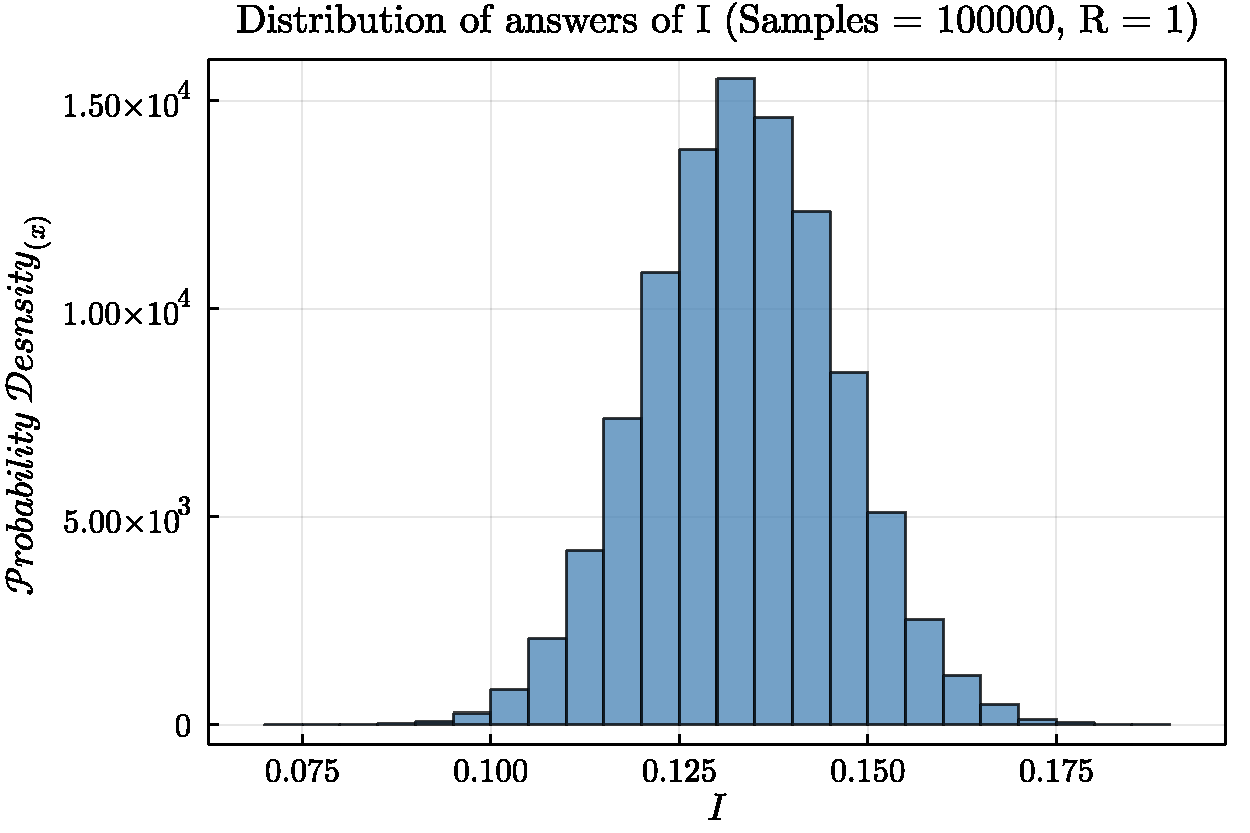
\includegraphics[scale = 0.25]{/Q2/IHistPlot}
        \label{fig:2.1}
        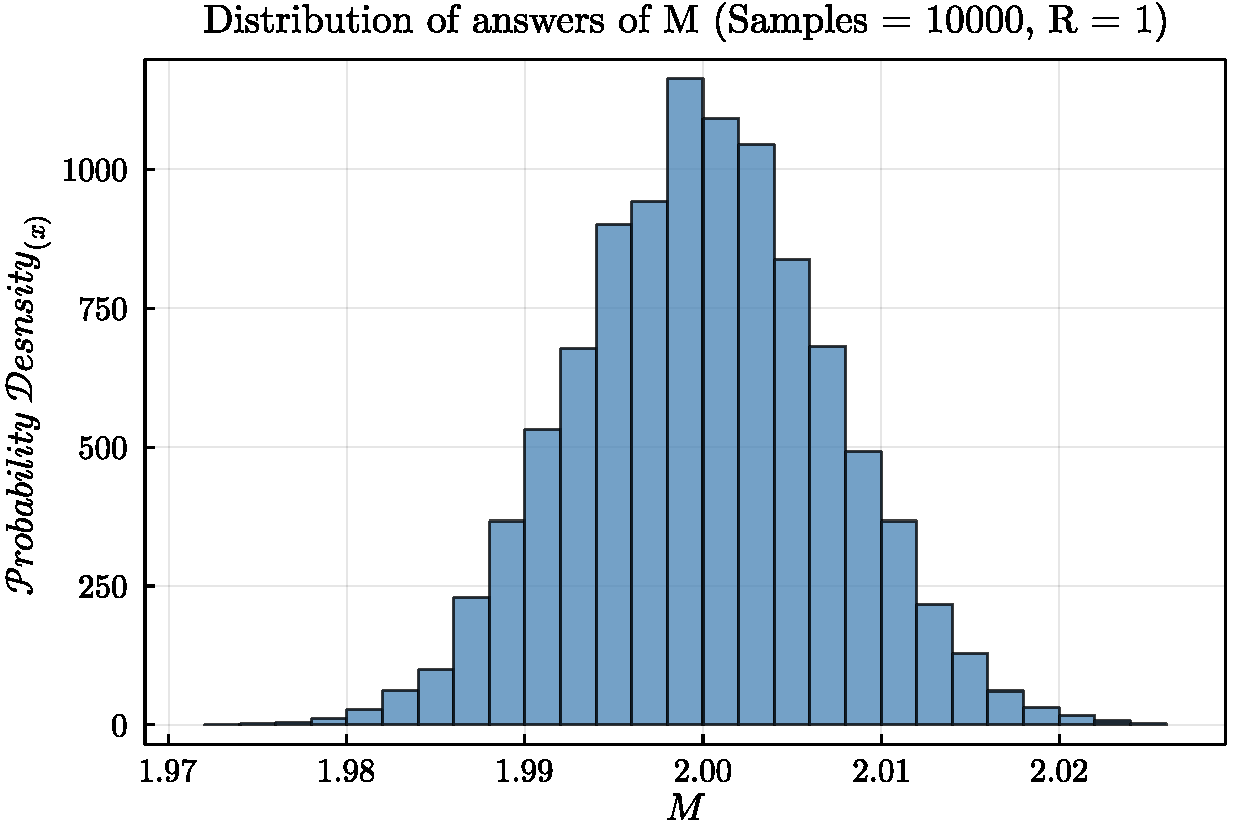
\includegraphics[scale = 0.25]{/Q2/MHistPlot}
        \label{fig:2.2}
        \caption{Distribution of answers of integration of I and M.}
    \end{figure}

    \pagebreak

    \section*{Problem 3}
    \textbf{Basic description:}

    In this problem, we want to create the Normal distribution
    by moving samples of the Uniform distribution in a span
    with various chances of movement and deploying the Metropolis algorithm.
    As we know the best distribution comes out with $a_r \approx 0.5$.
    So we draw a distribution with $a_r \approx 0.5$.
    Then, we will show the relation between $\Delta$ and $a_r$.
    And finally, we will show the Auto Correlation and Correlation length.
    The Correlation length will come out by finding the exponent of the Auto Correlation.

    \textbf{The results:}

    \begin{figure}[!htb]
        \centering
        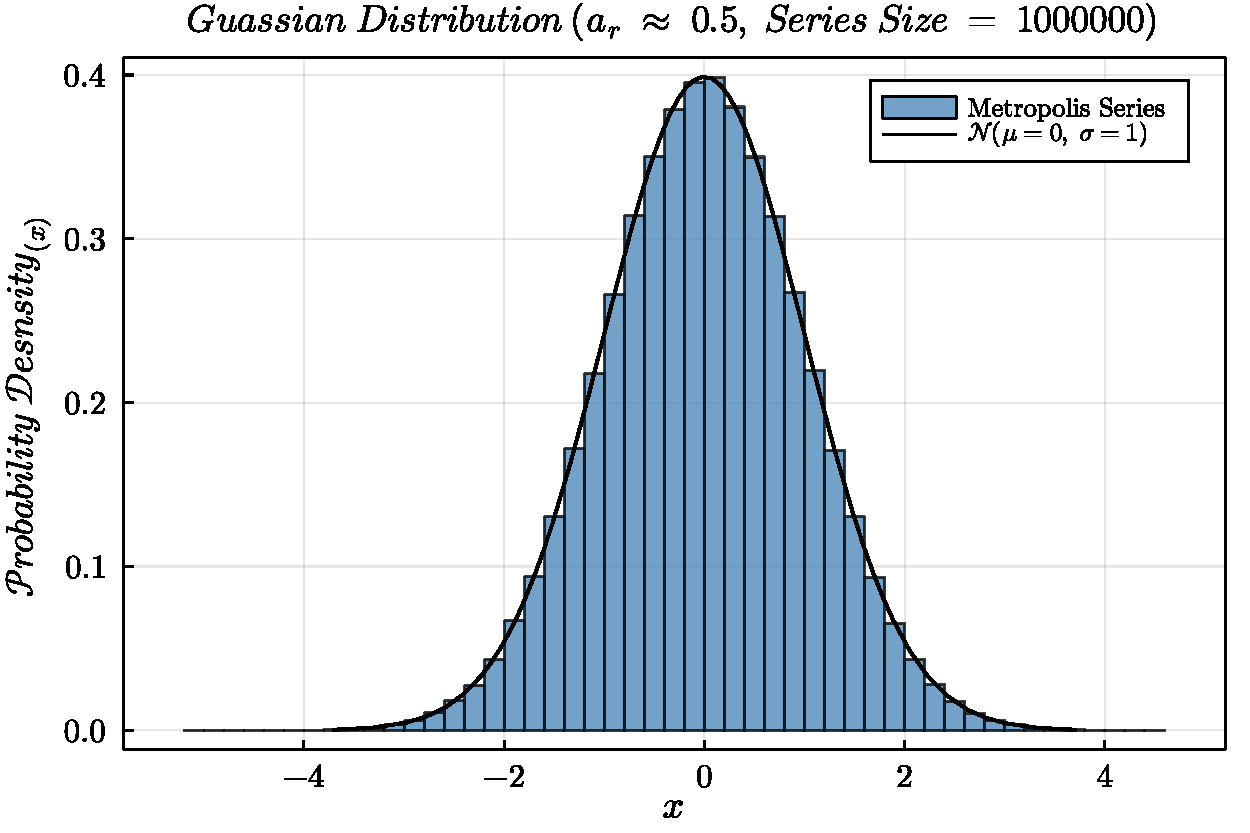
\includegraphics[scale = 0.4]{/Q3/NormalHist}
        \label{fig:3.1}
        \caption{Metropolis Normal Distribution with $a_r \approx 0.5$.}
    \end{figure}

    \begin{figure}[!htb]
        \centering
        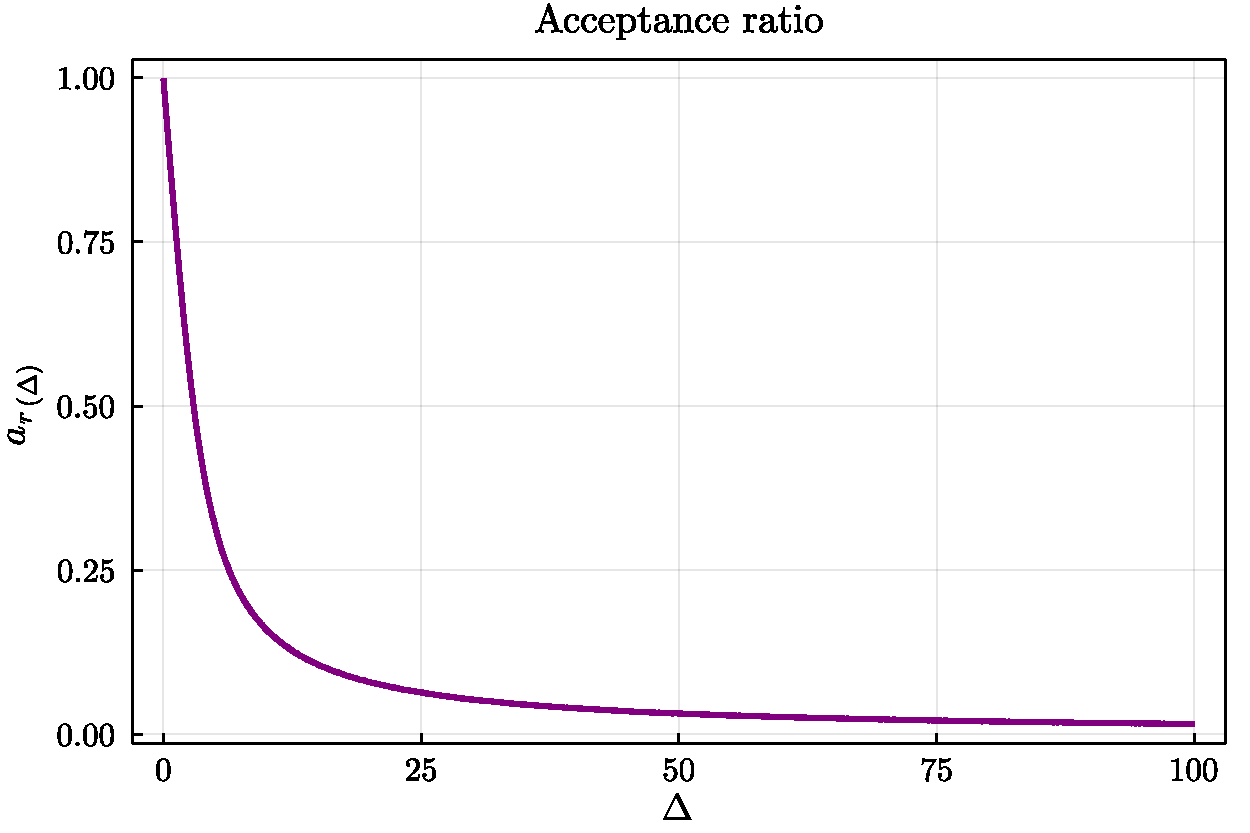
\includegraphics[scale = 0.4]{/Q3/AcceptanceRatio}
        \label{fig:3.2}
        \caption{Acceptance Ratio plot.}
    \end{figure}

    \begin{figure}[!htb]
        \centering
        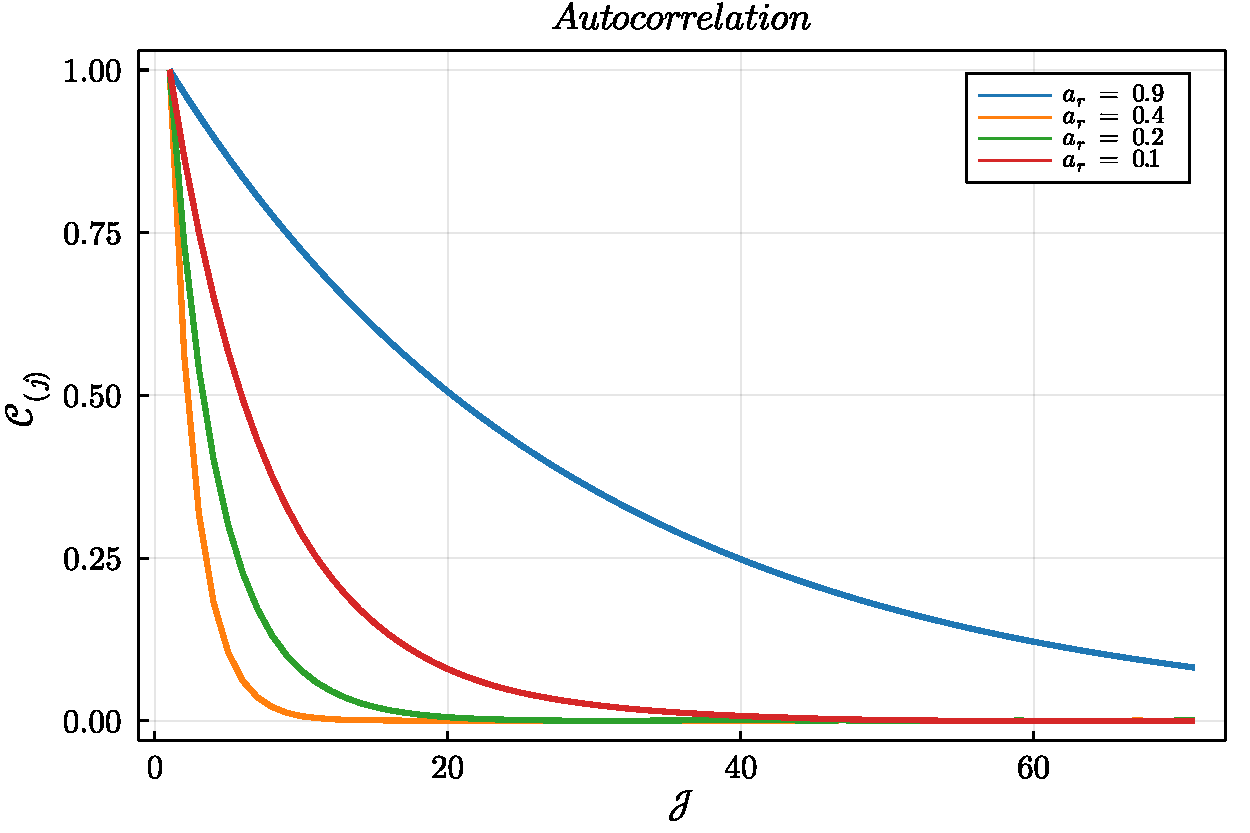
\includegraphics[scale = 0.3]{/Q3/Autocorrelation1}
        \label{fig:3.3}
        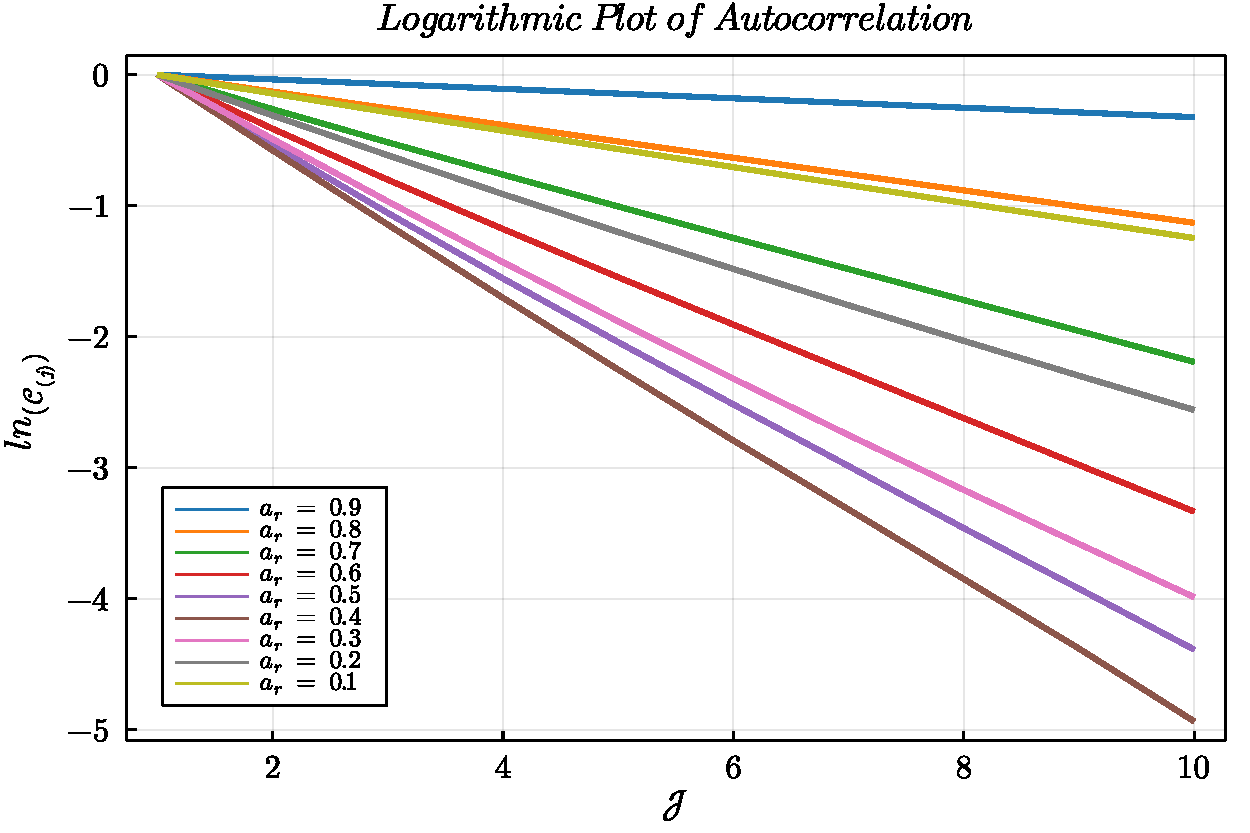
\includegraphics[scale = 0.3]{/Q3/Autocorrelation2}
        \label{fig:3.4}
        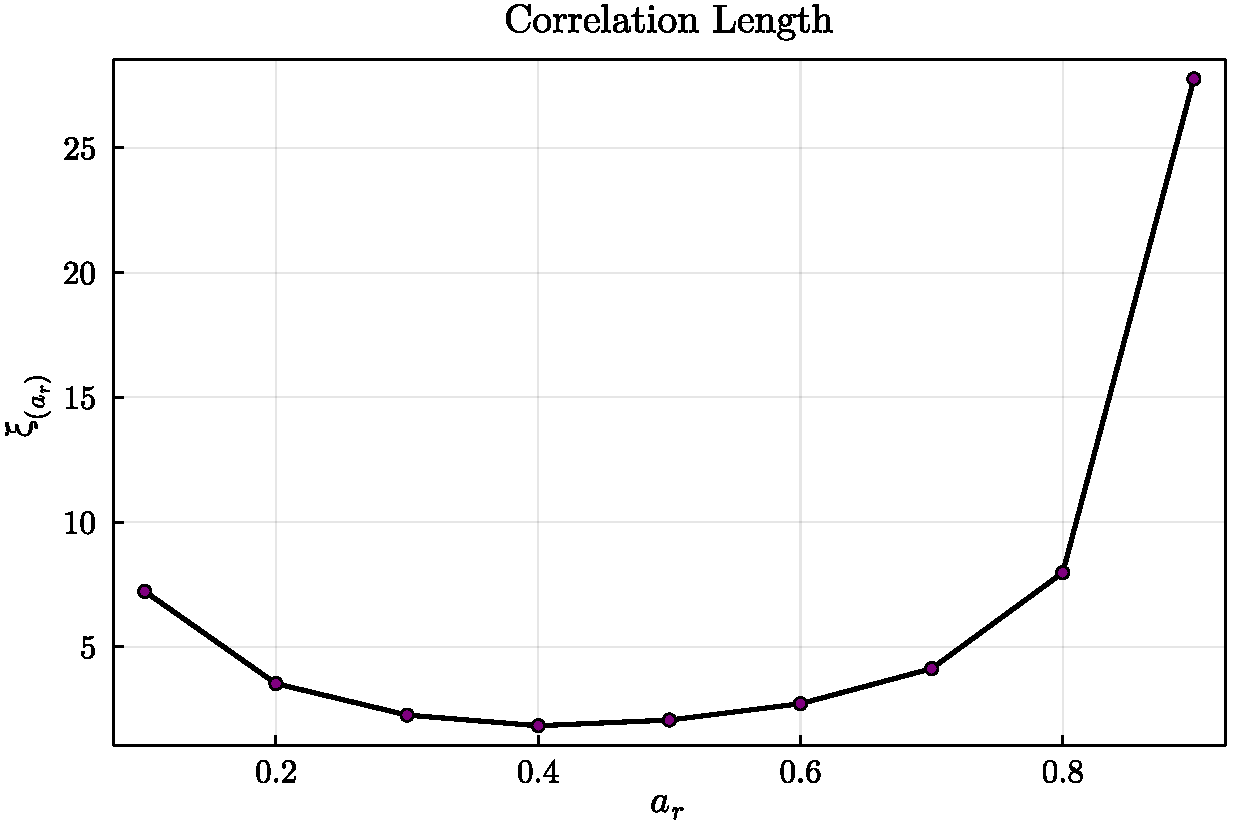
\includegraphics[scale = 0.3]{/Q3/CorrelationLength}
        \label{fig:3.5}
        \caption{Auto correlation and Correlation Length Plot.}
    \end{figure}

    \pagebreak

    \centering
    \textbf{The whole data I gathered is in \href{https://github.com/shahmari/ComputationalPhysics-Fall2021/tree/main/ProblemSet7/Data}{this link}}

    Thanks for watching :)
\end{document}